\chapter{Project Development}
In this chapter, the parts that compose this project as well as their context are shown. Also, some experiments are demonstrated for comparison with different parameters that have been used throughout the development of this thesis' project.

\section{Inputs and Outputs}
In previous chapters, it has been specified that this algorithm takes an text input and, according to its contents, a message is shown as an output. The breakdown is as follows.
\subsection{Inputs}
The input that is given is cleaned up and tokenized -- as shown in the previous chapter --, , this is then added to an internal corpus that has weights set for every word in it, effectively working as scores. Every word has a different score in every label, whether it is positive or negative. This score is added up and the highest final score will be the one that the algorithm will detect as the most probable for the text input. However, this has its caveats, small sentences are more likely to be miscategorized because one word can have different applications in the scope of this project, for a more accurate analysis a longer sentence must be written.
\subsection{Outputs}
Depending on the final score, the algorithm will choose a random sentence related to the detected sentiment, this is, as of the time of writing, very rudimentary, but the fact that it's built in Python this can be a building block for a more robust, context-conscious, reply system.

\section{Interface}
Originally, \textit{Ren'py}\footnote{An open-source Python framework focused mostly in the development of visual novels and other videogame formats. \url{https://www.renpy.org/}} was the chosen framework for this project's interface to work with, but -- unfortunately for the proposed usage -- it only works with Python 2.7, which makes it incompatible with TensorFlow 2.0. Making a bridge between Python 2 and 3 would inevitably generate more issues that would take more time to solve, so it was scrapped in favor of the \textit{pygame} library.
\pagebreak

\begin{figure}[!h]
	\centering
	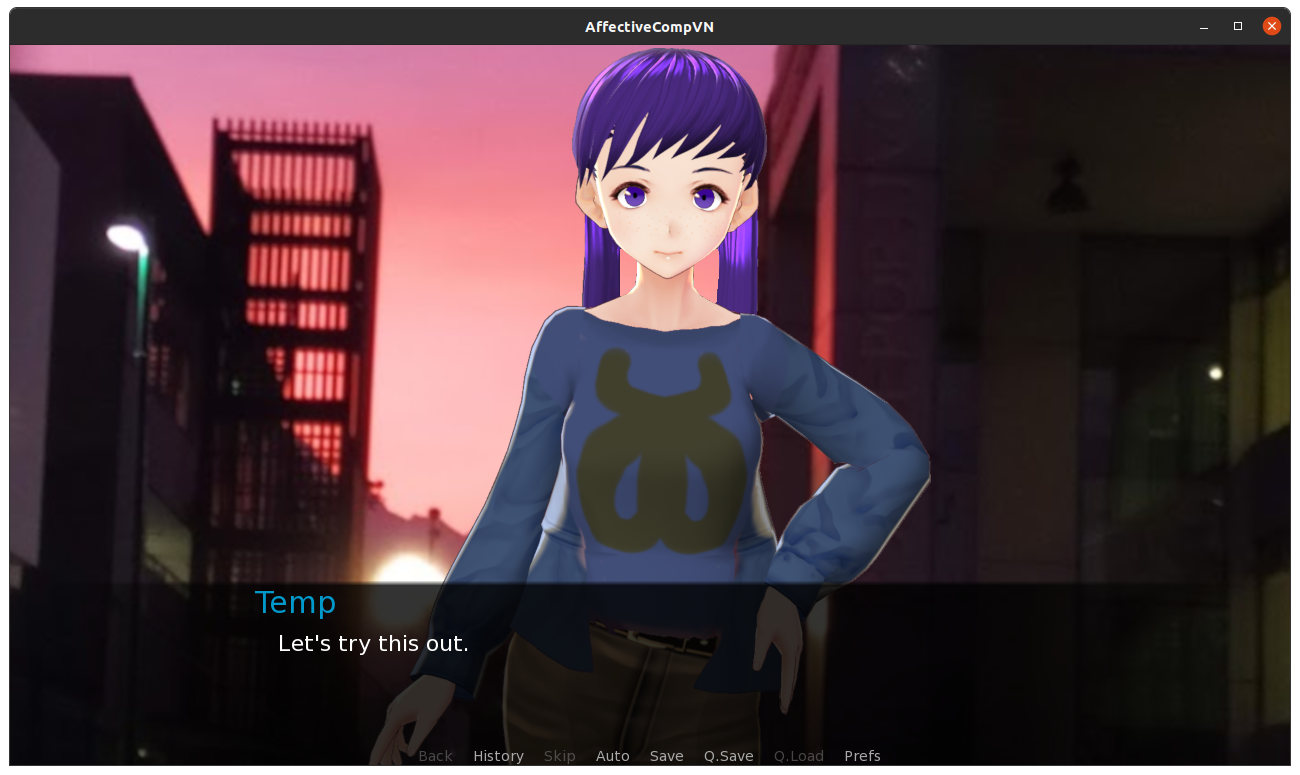
\includegraphics[scale=0.3]{Ren'py}
	\caption{First version of the interface using Ren'py.}
	\label{fig:renpy_test_1}
\end{figure}
\begin{figure}[!h]
	\centering
	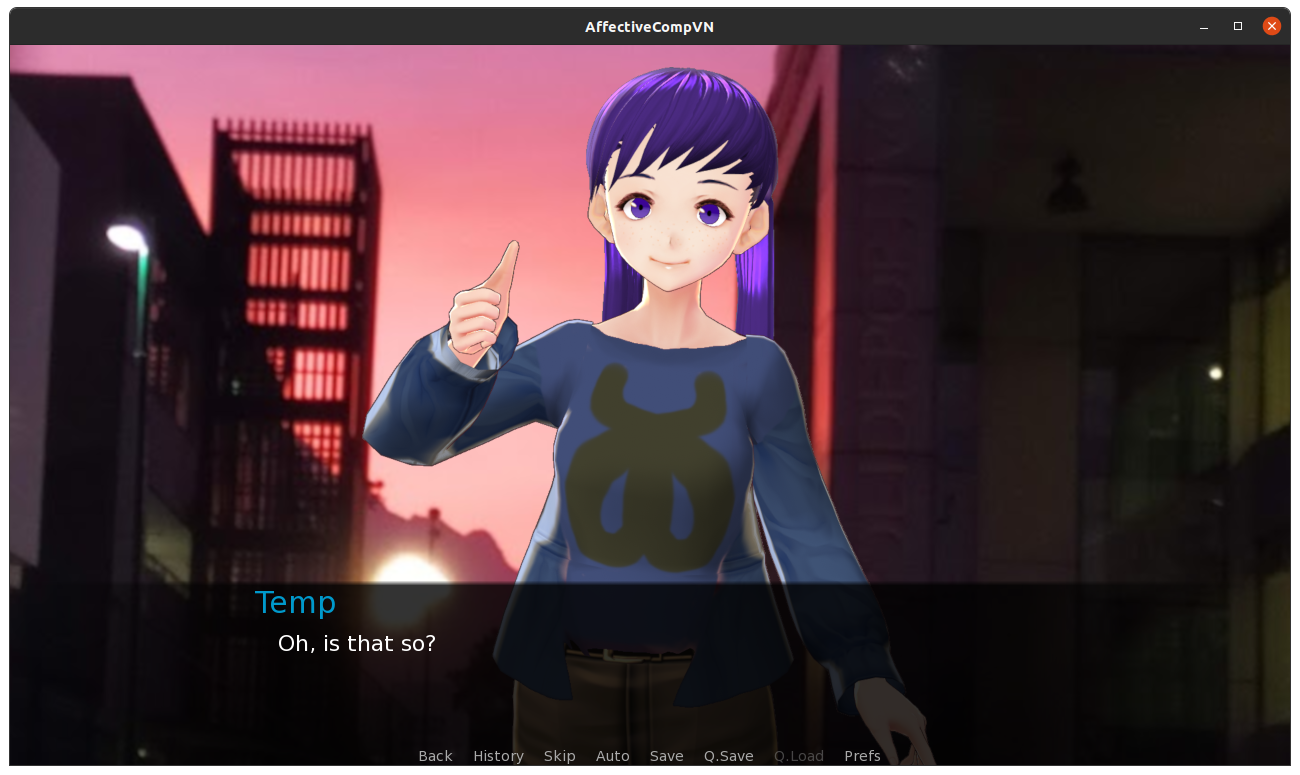
\includegraphics[scale=0.3]{Ren'py_2}
	\caption{Reacting positively to text in the ``Good'' category.}
	\label{fig:renpy_test_2}
\end{figure}

The current interface is a hybrid between a Pygame screen, where the assistant appears to react to the input, and the console, where a person can input text to be analyzed.

\subsection{Assistant}
As for the character that is being used, it also has gone through some changes. Originally the idea was to make a low-poly character render to work with, but since 3D modeling-from-scratch skills exceed the scope of this paper, an alternative software was selected instead. Namely \textit{VRoid}.\\
The main purpose for this assistant is to make people feel like it is her that they are talking to and not to some faceless machine, while also making it easier to the eyes. A more realistic, less animated style could have been used, but a friendly, less prone to uncanny valley approach to the design was opted for with this in mind.
\begin{figure}[!bht]
	\centering
	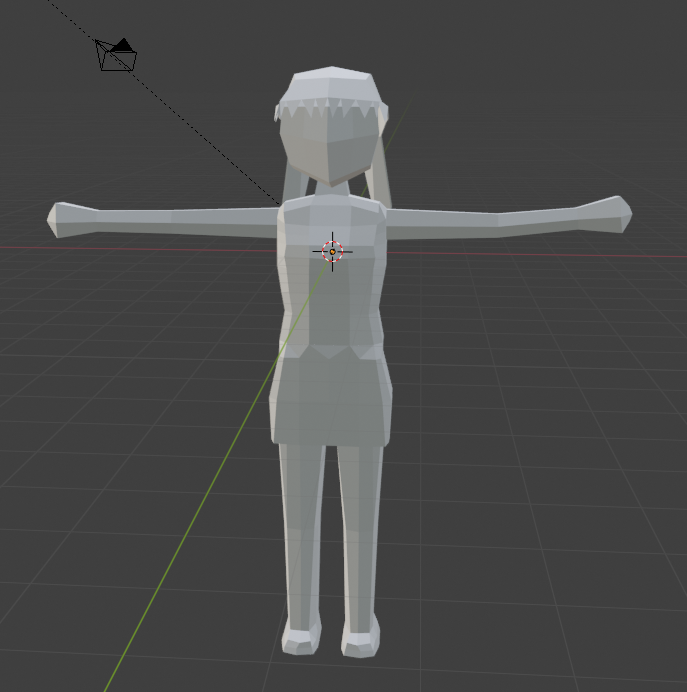
\includegraphics[scale=.5]{Assistant_1}
	\caption{First attempt at 3D modeling an assistant.}
	\label{fig:assistant1}
\end{figure}
\begin{figure}[!bht]
	\centering
	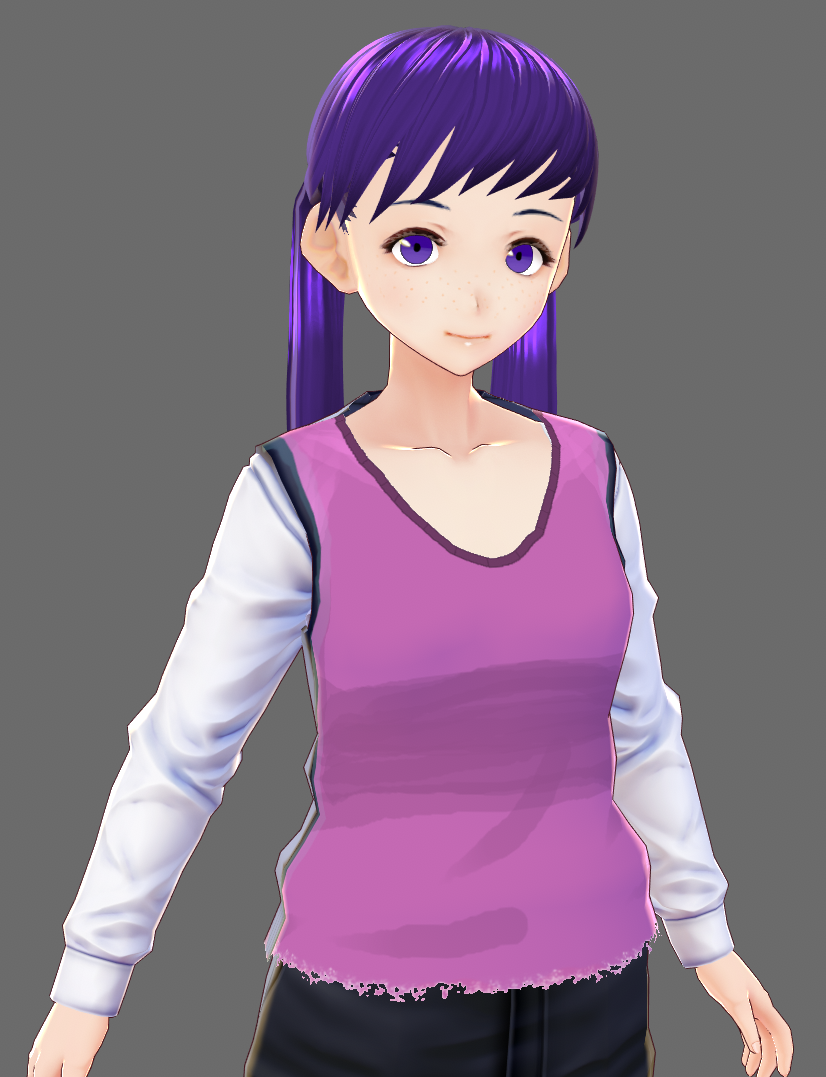
\includegraphics[scale=.25]{Assistant_2}
	\caption{Assistant Ver. 2, now using VRoid.}
	\label{fig:assistant2}
\end{figure}
\begin{figure}[!bht]
	\centering
	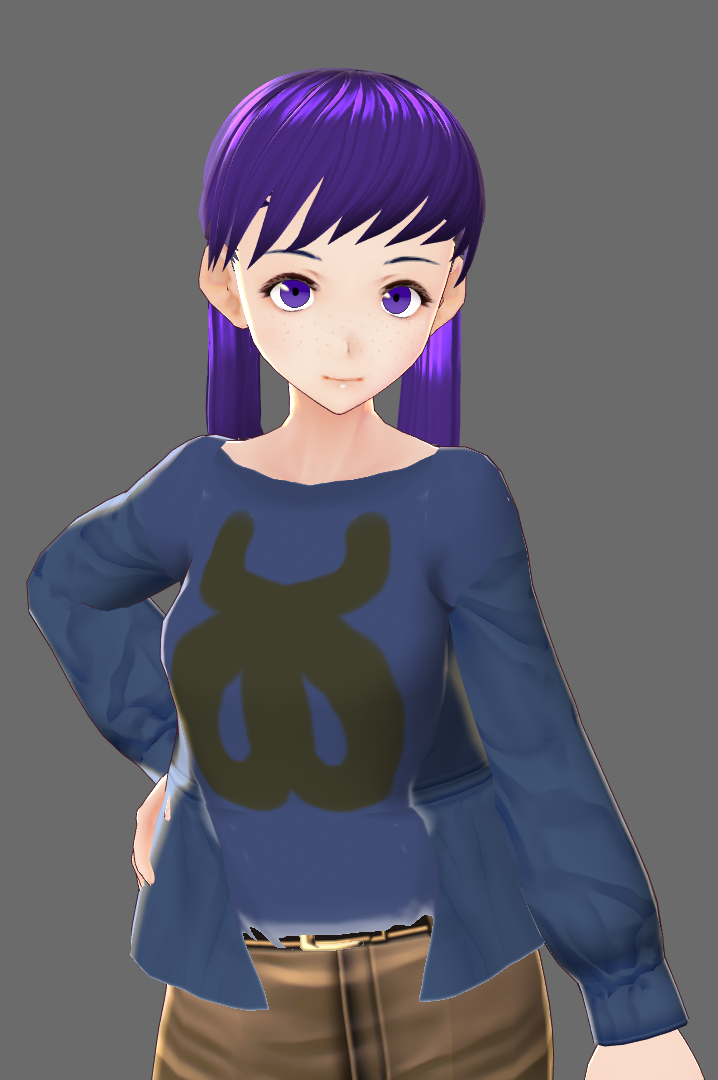
\includegraphics[scale=.25]{Assistant_3}
	\caption{Assistant Ver. 3, the current design.}
	\label{fig:assistant3}
\end{figure}
\pagebreak
\section{Experiments}
In this section, the evolution of this project is shown as experiments with varying modules and datasets with the respective accuracy and loss graphs.
\subsection{Experiment 1 / May 2020}
In the first version of this project, only one dataset was used, and the stemmer was not yet fully implemented.
\begin{table}[!h]
	\caption{Experiment 1's defining characteristics. Version link: \url{https://github.com/Alex-Ego/Affective-Computing-VN/tree/d4945b4bb506e0a6a0b6b3ad576d48f95cb745c4}}
	\vspace{0.5cm}
	\centering
	\begin{tabular}[t]{|l|l|}
	\hline
		Datasets Used & 1: \citet{d1}
	\\ \hline
		NLTK Usage & Only Tokenizer and Stopwords
	\\ \hline
		Epochs & 25
	\\ \hline
		Type of Neural Network & LSTM, 2 layers
	\\ \hline
	\end{tabular}
\end{table}
\\
\begin{figure}[!h]
	\centering
	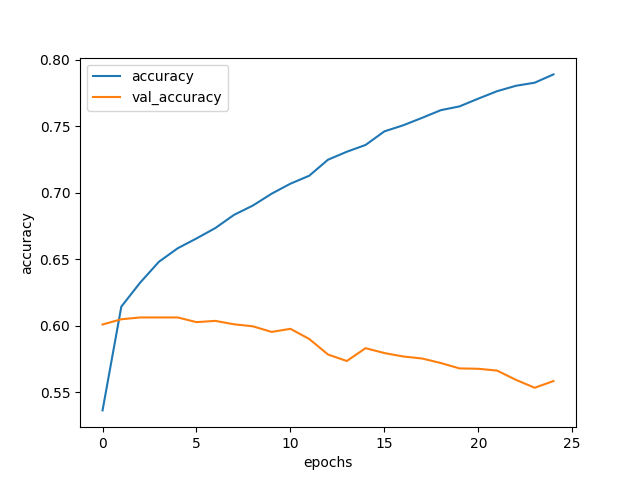
\includegraphics[scale=0.8]{Accuracy 2020-05}
	\caption{Accuracy Graph of the Algorithm Training on May 2020}
	\label{fig:accuracy2020}
	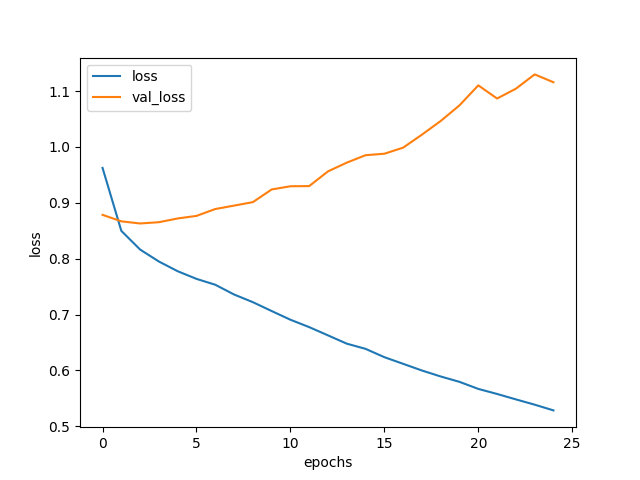
\includegraphics[scale=0.8]{Loss 2020-05}
	\caption{Loss Graph of the Algorithm Training on May 2020}
	\label{fig:loss2020}
\end{figure}
\pagebreak
\subsection{Experiment 2 / July 2021}
This second version, modified much later, does not have a lot of improvement over the last one, but the stemmer was fully deployed, a new dataset was used in tandem with the previous one, and the input is being properly filtered.
\begin{table}[!h]
	\caption{Experiment 2's defining characteristics. Version link: \url{https://github.com/Alex-Ego/Affective-Computing-VN/tree/7225434fc88b808e818c8681fc85e82937373db1}}
	\vspace{0.5cm}
	\centering
	\begin{tabular}[t]{|l|l|}
	\hline
		Datasets Used & 2: \citet{d1} and \citet{d2}
	\\ \hline
		NLTK Usage & Yes
	\\ \hline
		Epochs & 25
	\\ \hline
		Type of Neural Network & LSTM, 2 layers
	\\ \hline
	\end{tabular}
\end{table}
\\
\begin{figure}[!h]
	\centering
	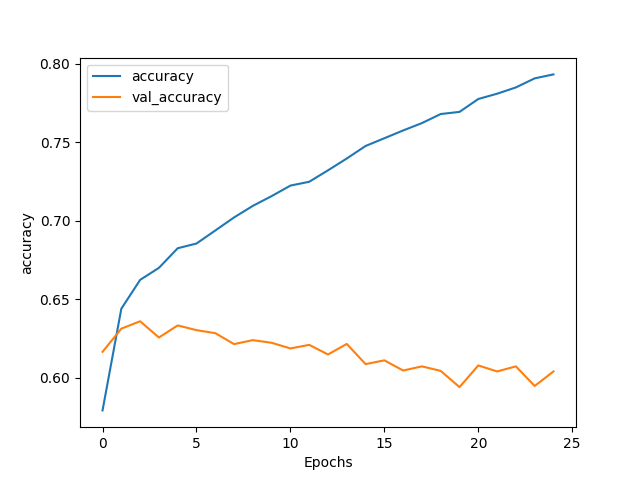
\includegraphics[scale=0.8]{Accuracy 2021-07}
	\caption{Accuracy Graph of the Algorithm Training on July 2021}
	\label{fig:accuracy2021-07}
	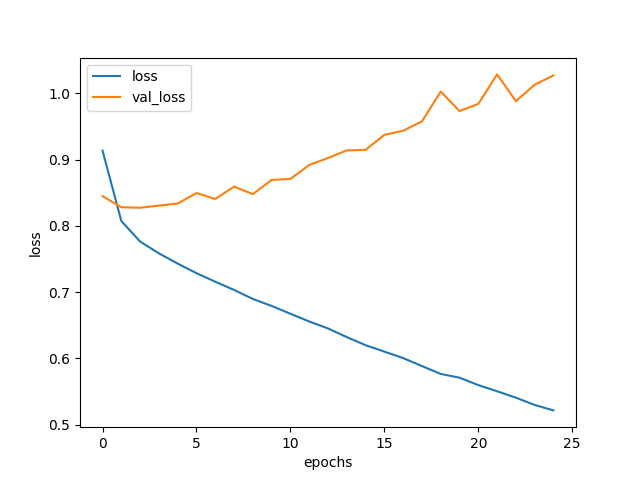
\includegraphics[scale=0.8]{Loss 2021-07}
	\caption{Loss Graph of the Algorithm Training on July 2021}
	\label{fig:loss2021-07}
\end{figure}
\pagebreak
\subsection{Experiment 3 / October 2021-1}
This version is allegedly the same that is being used today, much better chances of being correct. Also has 
\begin{table}[!h]
	\caption{Experiment 3's defining characteristics.}
	\vspace{0.5cm}
	\centering
	\begin{tabular}[t]{|l|l|}
	\hline
		Datasets Used & 3: \citet{d1}, \citet{d2} and \citet{d3}
	\\ \hline
		NLTK Usage & Yes
	\\ \hline
		Epochs & 30
	\\ \hline
		Type of Neural Network & LSTM, 2 layers
	\\ \hline
	\end{tabular}
\end{table}
\\
\begin{figure}[!h]
	\centering
	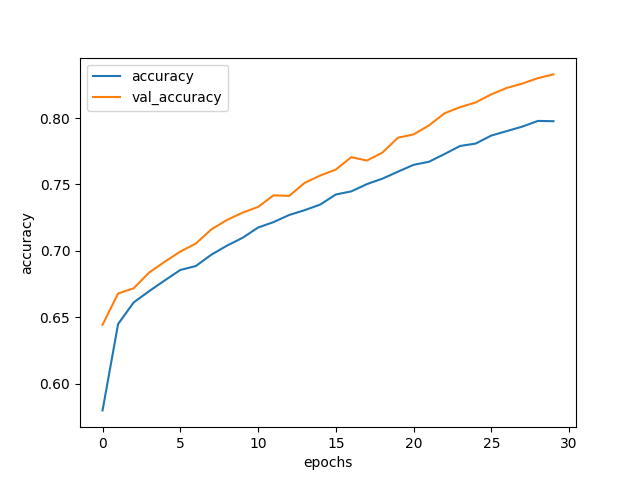
\includegraphics[scale=0.8]{Accuracy 2021-10}
	\caption{Accuracy Graph of the Algorithm Training on October 2021}
	\label{fig:accuracy2021-10}
	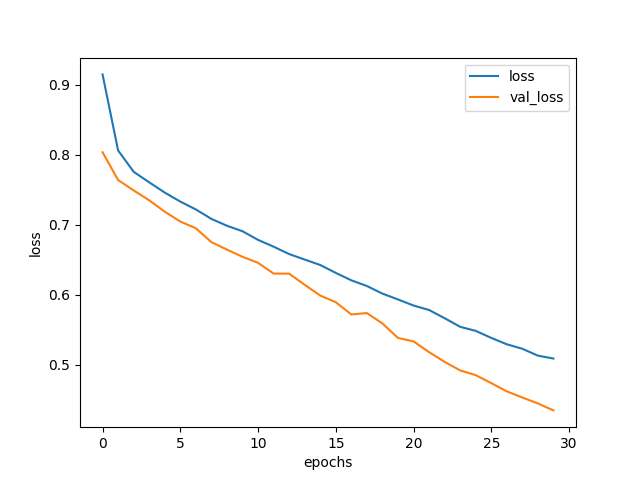
\includegraphics[scale=0.8]{Loss 2021-10}
	\caption{Loss Graph of the Algorithm Training on October 2021}
	\label{fig:loss2021-10}
\end{figure}


